\documentclass[11pt,parskip=half]{scrartcl}
\usepackage[utf8]{inputenc} 
\usepackage[T1]{fontenc} 
\usepackage{lmodern} 
\usepackage[english]{babel} 
\usepackage{amsmath} 
\usepackage{graphicx}
\usepackage{datatool}
\usepackage{hyperref}
\usepackage{listings}
\usepackage{color}

% Datatool settings
\catcode`\^^I=12 %
\DTLsetseparator{	}% <-- tab character

\begin{document}

\author{Rasmus Sjostrom, John Herrlin}
\title{1DV702}
\subtitle{Assignment \#3, Group J}
\date{\today}
\maketitle

\tableofcontents
\newpage

\section{Part I - Segmentation Architecture Fundamentals}
\subsection{Hub vs Switch Behavior}

\subsubsection{Hub Behavior}
Full-duplex allows for bidirectional communication, just as half-duplex but with a big difference. Full-duplex lets traffic flow in both direction simultaneously, which is not true for half-duplex where the traffic can only flow in one direction at a given time. Because full-duplex separates incoming and outgoing traffic, it is not affected by collisions as the channels are separate.

Auto-negotiation is used between devices to come up with common, acceptable communication characteristics. This includes things like link speed, duplex mode and transmission rates. Normal Link Pulse is a sort of idle communication used to register the presence of a connected device. These pulses can form code words which are used to assist in the agreement of previously mentioned communication characteristics.

When monitoring the traffic from machine M in Wireshark, all traffic can be seen. This is due to the behavior of the Hub; a hub simply duplicates all packets on all ports, regardless of what device the packet was intended for.

\subsubsection{Switch Behavior}
\begin{figure}[!ht]
\begin{itemize}
\item Laptop1: 	 74:d0:2b:08:e8:c4 - 10.0.0.2
\item Laptop2:   00:21:cc:c2:83:48 - 10.0.0.3
\item PC:	  	 00:1a:a0:6a:08:f2 - 10.0.0.4
\caption{Hardware addresses and static IP configuration.}
\end{itemize}
\end{figure}
\textbf{Experiment 1:}\\
No traffic from the pings were captured since the switch only forwards
the traffic to the destination host.

Since we set all the MAC to IP mappings statically in each host, there
was no need for any of them to send any ARP traffic. Thus, there were no
ARP traffic in the capture.

\textbf{Experiment 2:}\\
As for the first experiment, the switch only forwards the ping traffic to
the destination host address and is not displayed in the capture. However since we did not assign the MAC to IP mapping statically this time, there
were ARP traffic shown in the capture for the second experiment.

\textbf{Conclusion:}\\
The difference between the captured traffic in experiment 1 and 2 were
the ARP traffic. Since we assigned the MAP to IP mappings in experiment 1
statically, there was no sign of any ARP traffic in that capture. While
in the experiment 2 capture file we could see the APR requests between the
two laptops from the capturing PC.

\subsubsection{Conclusions}
The hub has only got one collision domain, therefore there is a bigger
chance for collisions. A switch on the other hand has one collision domain
per port. This leads to reduced collisions.
  
When it comes to broadcast traffic, the switch acts the same way as a hub.
Otherwise, the switch only forwards frames to the destination device. This
can be seen in the previous experiment, where we could see the ARP request
but no response was shown to the third PC.

\subsection{VLAN}
\subsubsection{Single Switch}
\textbf{Experiment 1:}\\
When both hosts were connected to the same VLAN, we could both ping each
other and the capturing PC could see the broadcast traffic generated by the
other laptop. None of these things were however not possible when the two
hosts were on different VLANs.
  
Assigning the same IP to two hosts on different VLANs does not cause any
issues what so ever since they are completely separated.

\textbf{Experiment 2:}\\
Communication between the two laptops on separate VLANs is not possible
since none of the hosts can reach the other hosts virtual network.

\subsubsection{Multiple Switches}
The two hosts connected to the different switches could not communicate or
see each others broadcasts. This is due to the fact that no trunking has
been configured in the switches.

\subsection{Spanning Tree}
\textbf{Examine the STP Default State:}\\
When clicking the 'Capture/Forward' button, we can see packets
starting from S6. This is the root bridge, which we then
confirmed by entering the CLI and ran the 'show spanning-tree'
command.

\textbf{Configure the root bridge:}\\
By switching to real time mode and entering the command
'spanning-tree VLAN 1 priority 4096' in the configuration
terminal in C1 we configured it to be the root bridge.

\textbf{Configure the Backup Root Bridge:}\\
When C2 is configured as the backup root bridge, the links
between C2 and the distribution layer are amber while the links
going from C1 are all green.

Figure 2 shows a screenshot of the finished Packet Tracer assignment.
\begin{figure}[!ht]
	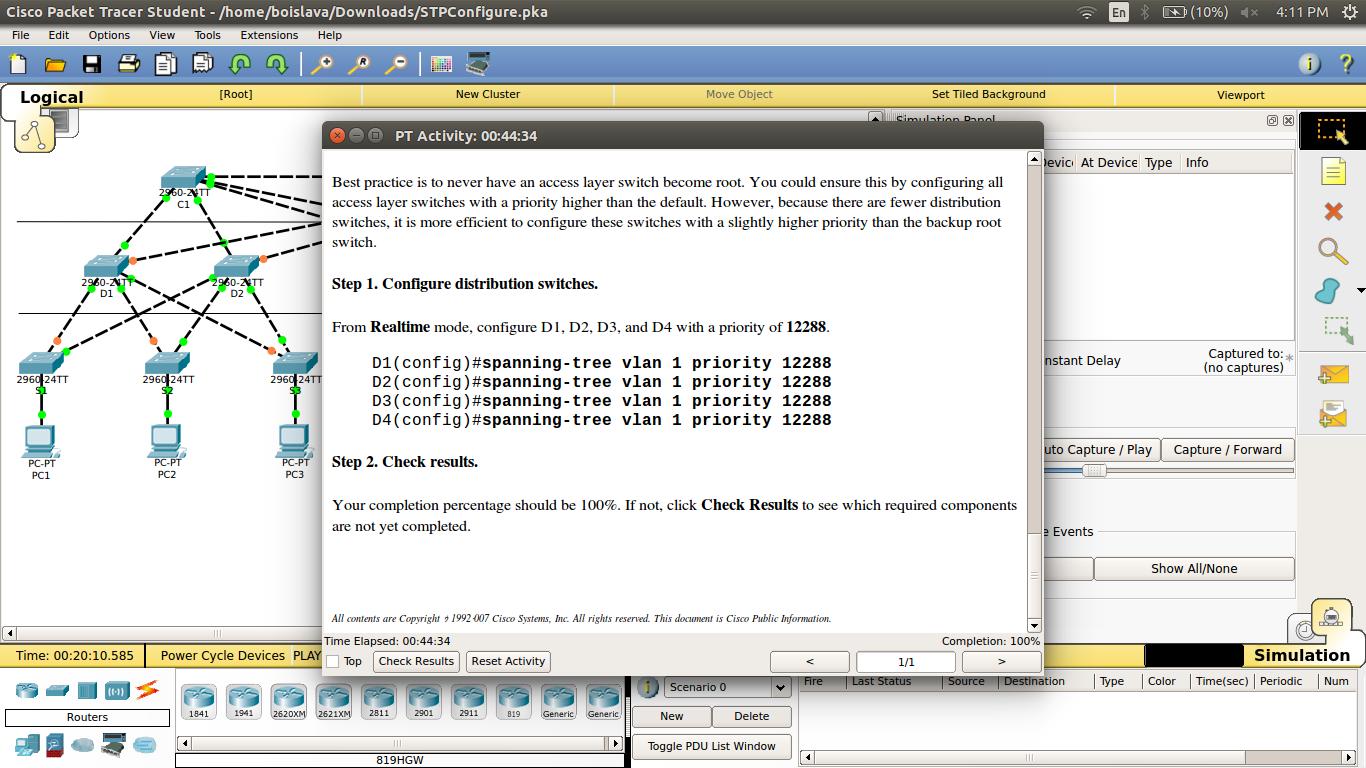
\includegraphics[width=1\textwidth]{configure-pt}
    \caption{Screenshot of the finished Packet Tracer assignment.}
\end{figure}

\newpage
\section{Part II - Addressing and Routing Architecture}

\subsection{IP Addressing}

We assigned the major network the IP address of 10.0.0.0, and then used the online
tool \href{http://vlsm-calc.net/}{vlsm-calc} to calculate and divide the network into 
subnets with proper address sizes. 

The networks labeled BACK1-5 in the topology in
fig. 3 are the backbone networks which connects each of the routers to each other as 
well as to the firewall and further on out on the Internet.

\begin{figure}[!h]
	\centering
    %fixme :: insert screenshot
    \caption{Topology of the Network}
\end{figure}

Thanks to sub-netting like this almost 0\% of the available address space on the
major network is used, and about 82\% in the subnets. This is shown in fig. 4

\begin{figure}[!ht]
	\centering
	\DTLloaddb{address-use}{address-use.tsv}
	\resizebox{.6\linewidth}{!}{\noindent\DTLdisplaydb{address-use}}
    \caption{Address Usage}
\end{figure}

\begin{figure}[!ht]
	\DTLloaddb{subnets}{subnet-table.tsv}
	\resizebox{1.1\linewidth}{!}{\noindent\DTLdisplaydb{subnets}}
    \caption{Network Information}
\end{figure}

\subsection{Routing}
Routing is done in the backbone networks and each one of the Mikrotik, Cisco CSR,
pfSense and Cisco ASA uses \href{https://en.wikipedia.org/wiki/Open_Shortest_Path_First}{Open Shortest Path First (OSPF)} to find routes and neighbors. Fig. 6 displays the routing table for all of the just mentioned devices respectively.

The NAT is however only configured in one place in the network, which is in the
Cisco ASA. This device is (as shown in the previous section) connected to the
Internet on one interface, and has a single point of entry into the network,
starting with the pfSense.

\begin{figure}[!ht]
	\centering
    %fixme
    \caption{Routing Tables}
\end{figure}

\section{Appendix: Configuration \& Additional Notes (Part II)}
This is section primarily contains lists of commands used to configure and manage
all the devices (apart from the pfSense which was configured via the web service),
as well as notes and general information about the networks that are related to all
of these devices. 

It also contains some related information about how to do some basic operations on some of the devices, such as printing routing tables etc.

This appendix is the documentation made to keep track and remember how each of the devices was configured throughout the second part of the assignment.

\subsection{{\bfseries\sffamily } Microtik}
\label{sec:org78e1204}

\begin{center}
\begin{tabular}{ll}
User & admin\\
Password & <BLANK>\\
\end{tabular}
\end{center}

\begin{center}
\begin{tabular}{lrlll}
Network & IP & CIDR & Netmask & Interface\\
\hline
BACK1 & 10.0.4.18 & /29 &  & ether1\\
BACK2 & 10.0.4.25 & /29 &  & ether2\\
PARENT & - & - & - & ether3\\
VLAN10 & 10.0.3.129 & /26 &  & VLAN10\\
VLAN20 & ? & ? &  & VLAN20\\
\end{tabular}
\end{center}

\begin{lstlisting}[basicstyle=\small, frame=single]
/interface vlan
add interface=ether3 name=vlan10 vlan-id=10
add interface=ether3 name=vlan20 vlan-id=20
/ip pool
add name=dhcp_pool1 ranges=10.0.3.130 - 10.0.3.190
/ip dhcp-server
add address-pool=dhcp_pool1 disabled=no interface=vlan10 name=dhcp1
/ip address
add address=10.0.3.129/26 interface=vlan10 network=10.0.3.128
add address=10.0.4.18/29 interface=ether1 network=10.0.4.16
add address=10.0.4.25/29 interface=ether2 network=10.0.4.24
/ip dhcp-server network
add address=10.0.3.128/26 dns-server=8.8.8.8 gateway=10.0.3.129
/routing ospf network
add area=backbone network=10.0.3.128/26
add area=backbone network=10.0.4.0/28
add area=backbone network=10.0.4.24/29
add area=backbone network=10.0.4.16/29
\end{lstlisting}

\begin{verbatim}
ip route
print
\end{verbatim}

\subsection{{\bfseries\sffamily } PfSense}
\label{sec:org08ed6ad}

\begin{center}
\begin{tabular}{ll}
User & admin\\
Password & pfsense\\
\end{tabular}
\end{center}

\begin{center}
\begin{tabular}{lrlll}
VLAN & IP & CIDR & Netmask & Interface\\
\hline
BACK1 & 10.0.4.17 & /29 & 255.255.255.248 & em3\\
BACK3 & 10.0.4.33 & /29 & 255.255.255.248 & em4\\
BACK4 & 10.0.4.42 & /29 & 255.255.255.248 & em0\\
PARENT & - & - & - & em1\\
VLAN50 & 10.0.3.1 & /25 &  & em1\\
VLAN60 & 10.0.3.193 & /26 &  & em1\\
Firefox & 10.0.4.49 & - & - & em2\\
\end{tabular}
\end{center}

\subsection{{\bfseries\sffamily } Cisco Router}
\label{sec:org4c9df29}

\href{https://github.com/jherrlin/dotfiles/blob/master/arch/helpme/.docs/cisco.org}{GH notes}

All interfaces need to be brought up manually.

\begin{center}
\begin{tabular}{lrlrl}
VLAN & IP & CIDR & Netmask & Interface\\
\hline
BACK3 & 10.0.4.34 & /29 & 255.255.255.248 & GigabitEthernet2\\
BACK2 & 10.0.4.26 & /29 & 255.255.255.248 & GigabitEthernet1\\
VLAN30 & 10.0.2.1 & /24 & 255.255.255.0 & GigabitEthernet3\\
VLAN40 & 10.0.0.1 & /23 & 255.255.254.0 & GigabitEthernet3\\
\end{tabular}
\end{center}


\begin{lstlisting}[basicstyle=\small, frame=single]
interface GigabitEthernet1
ip address 10.0.4.26 255.255.255.248
no shut
exit

interface GigabitEthernet2
ip address 10.0.4.34 255.255.255.248
no shut
exit

interface GigabitEthernet3
no ip address
ip access-group 101 in
negotiation auto

interface GigabitEthernet3.30
  encapsulation dot1Q 30
  ip address 10.0.2.1 255.255.255.0
  ip access-group 130 in

interface GigabitEthernet3.40
  encapsulation dot1Q 40
  ip address 10.0.0.1 255.255.254.0

ip dhcp pool vlan30
  network 10.0.2.0 255.255.255.0
  default-router 10.0.2.1
  dns-server 8.8.8.8

router ospf 10
  network 10.0.0.0 0.0.0.255 area 0
  network 10.0.0.2 0.0.0.255 area 0
  network 10.0.4.24 0.0.0.255 area 0
  network 10.0.4.32 0.0.0.255 area 0
\end{lstlisting}

\begin{verbatim}
wr mem // Write config
conf m // Load config 
\end{verbatim}

\subsection{{\bfseries\sffamily } Cisco ASA}
\label{sec:org441b035}

\begin{center}
\begin{tabular}{lllll}
VLAN & IP & CIDR & Netmask & Interface\\
\hline
internet & DHCP &  &  & GigabitEthernet0/1\\
BACK4 & 10.0.4.41 & /29 & 255.255.255.248 & GigabitEthernet0/1\\
\end{tabular}
\end{center}

\begin{lstlisting}[basicstyle=\small, frame=single]
interface Gigabitethernet0/0
  no shut
  nameif INTERNAL
  security-level 100
  ip address 10.0.4.41 255.255.255.248

interface GigabitEthernet0/1
  no shut
  nameif EXTERNAL
  security-level 100
  ip address dhcp setroute

object network internal-external-nat
  subnet 10.0.4.40 255.255.255.248
  nat (internal,external) dynamic interface

policy-map global_policy
  class inspection_default
  inspect icmp

router ospf 10
  network 10.0.4.40 255.255.255.248 area 0
  network 10.0.4.40 0.0.0.255 area 0
  network 0.0.0.0 0.0.0.0 area 0
  log-adj-changes
  default-information originate always

object network internal-nat
  subnet 10.0.0.0 255.0.0.0
  nat (INTERNAL,EXTERNAL) dynamic interface

object network external-nat
  subnet 0.0.0.0 0.0.0.0
  nat (INTERNAL,EXTERNAL) dynamic interface

same-security-traffic permit inter-interface
mtu INTERNAL 1500
mtu EXTERNAL 1500
\end{lstlisting}

Show routes

\begin{verbatim}
show route
\end{verbatim}

Show ASP table routing

\begin{verbatim}
show asp table routing
\end{verbatim}

\subsubsection{{\bfseries\sffamily } Resources}
\label{sec:org985a263}

\href{https://www.speaknetworks.com/enable-icmp-inspection-to-allow-ping-traffic-passing-asa/}{Allow ICMP}

\subsection{{\bfseries\sffamily } Config light hosts}
\label{sec:org6f323cf}
\subsubsection{{\bfseries\sffamily } Firefox OS}
\label{sec:org7fa7c9d}

This is the commands to set a static IP address on the Firefox OS hosts.

\begin{verbatim}
sudo su
ifconfig eth0 10.0.4.50
route add default gw 10.0.4.1
\end{verbatim}

\subsubsection{{\bfseries\sffamily } Tiny clients}
\label{sec:orgdc14fee}

To get an IP address from the DHCP server.

\begin{verbatim}
ip dhcp -r
show ip
\end{verbatim}

\end{document} 
